%%%%%%%%%%%%%%%%%%%%%%%%%%%%%%%%%%%%%%%%%%%%%%%%%%%%%%%%%%%%%%%%%%%%%%%%%%%%%%%%
% data_set.tex:
%%%%%%%%%%%%%%%%%%%%%%%%%%%%%%%%%%%%%%%%%%%%%%%%%%%%%%%%%%%%%%%%%%%%%%%%%%%%%%%%
\chapter{Background Samples}
\label{data_set_chapter}
\begin{figure}[!htbp]
    \centering
    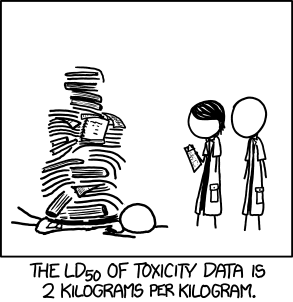
\includegraphics[width=.4\textwidth]{figures/DataSets/DataDeadly.png}
    \caption[]{fortunately for us, we do not need to make paper copies of all the simulated events we have. \cite{xkcdComic}}
    \label{fig:DataDeadly}
\end{figure}{}
Studies of \Ztoll, such as \phistar, are useful due to the clarity of the signal, with over 99.5\% of the data being signal events($\Ztoee$) after selection has been applied. The majority of background events involve a Z, such as ZZ, WZ, as well as \Ztotautau. These along with the other backgrounds that do not contain a Z are used are shown in Table~\ref{table:bgFrac}.
\begin{table}[ht]
    \centering
    \caption{
        Data sample composition as a percentage of the total and as a percentage of just the backgrounds. These represent the samples that were used for unfolding
    }
    \label{table:bgFrac}
    \begin{tabular}{ | l |l | l | r | r |}
        \hline
        Process & Generator & $\sigma$ (pb)&   ratio to signal & \% background \\ \hline
        \ttbar & Madgraph & 23.64& 0.0017 & 27.7 \\ \hline
        $ZZ$ & Pythia6 & 17.7& 0.0012 & 19.9 \\ \hline
        $W^{\pm}Z$& Pythia6 &33.21 & 0.0012 & 19.7 \\ \hline
        $Z \rightarrow \tau^+\tau^-$& Powheg&1966.7 & 0.0009 & 14.9 \\ \hline
        QCD Multi-jet \& $W^{\pm}+\text{jets}$& N.A.&N.A. & 0.0006 & 10.0 \\ \hline
        $W^+W^-$& Pythia6 & 54.84&0.0003 & 5.2 \\ \hline
        $tW^- \& \overline{t}W^+$& Powheg&22.1 & 0.0002 & 2.7 \\ \hline
    \end{tabular}
\end{table}

\begin{figure}
    \centering
    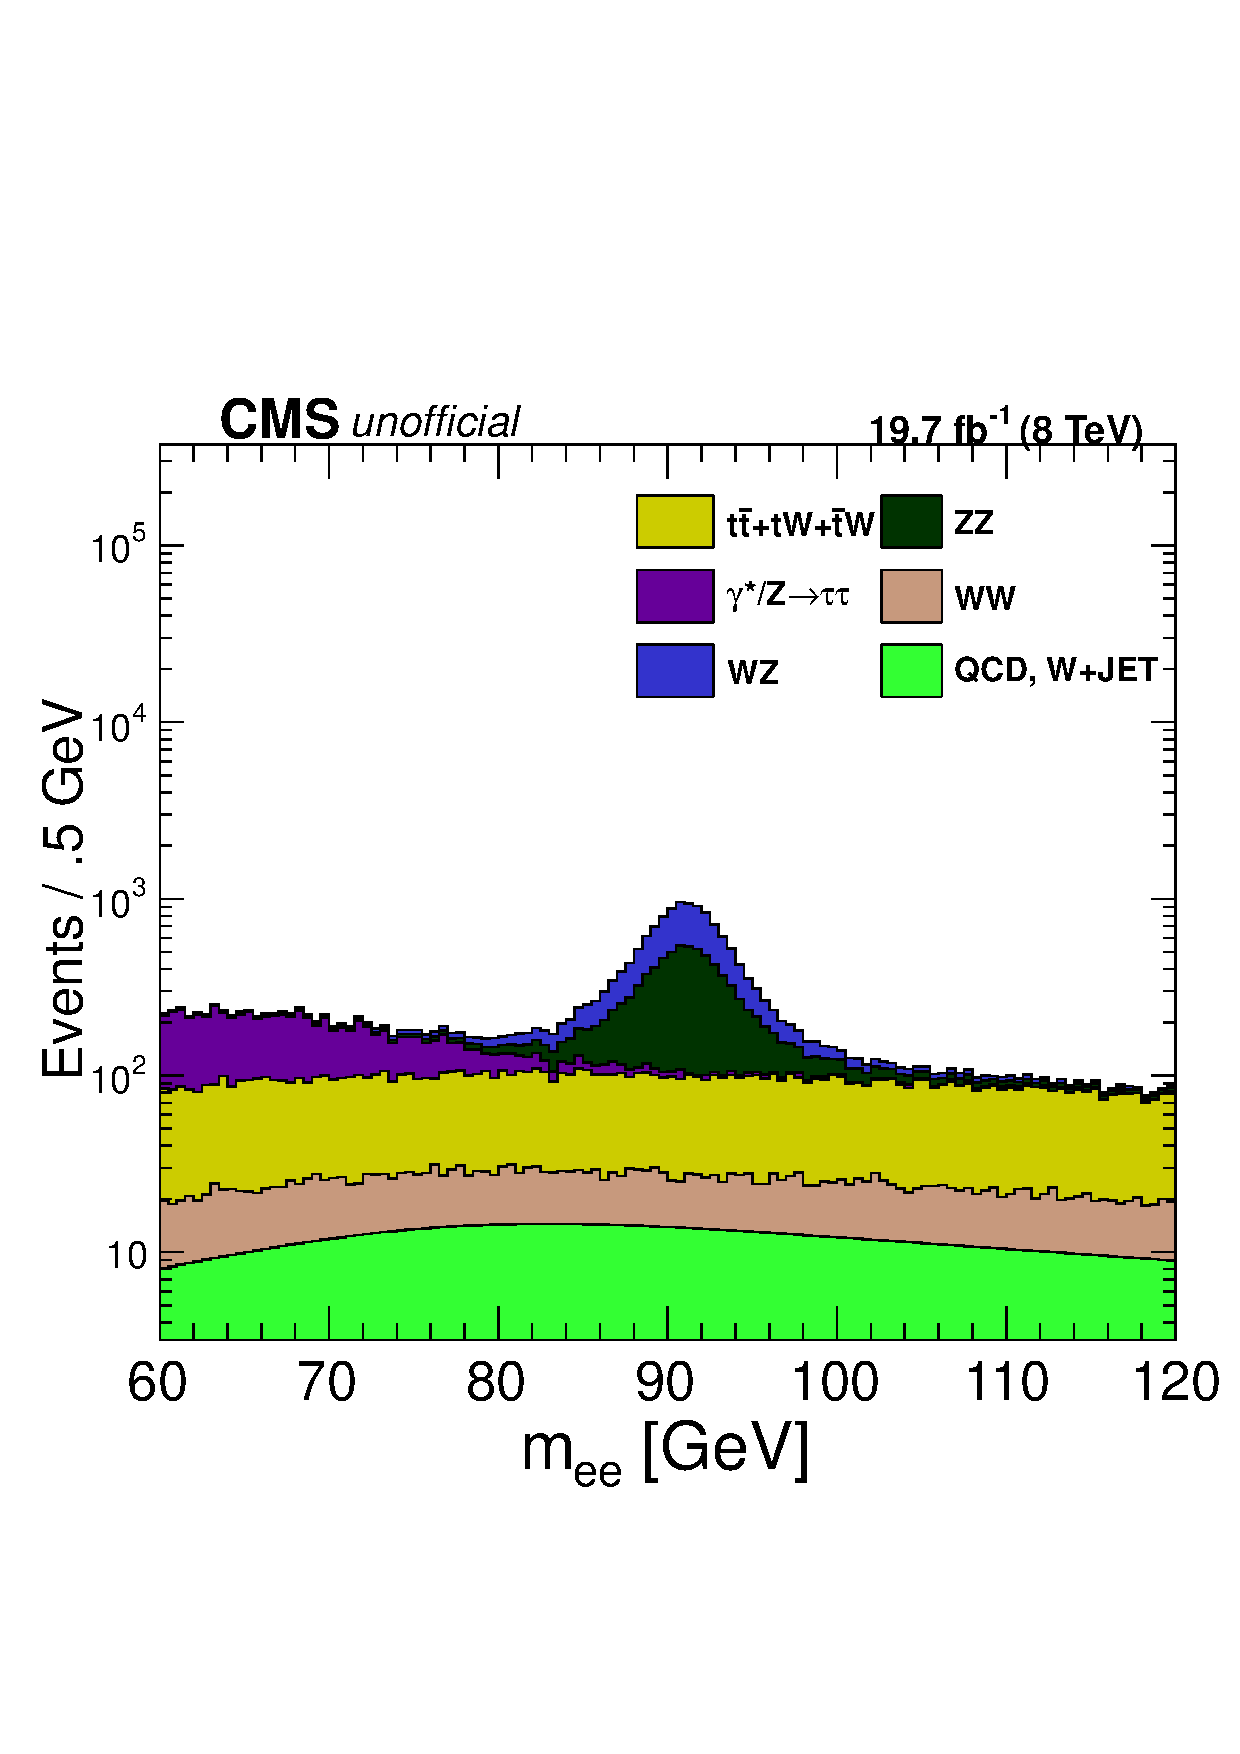
\includegraphics[width=\textwidth]{figures/DataSets/BGSMPlots.pdf}
    \caption[The \mee distribution of the background samples used]{A plot of the center of mass values of all the backgrounds stacked. With the exception of the ZZ and WZ all the Backgrounds have a relatively flat distribution.}
    \label{fig:BackgroundSM}
\end{figure}
All analyzed backgrounds were predicted via simulation with the exception of QCD Multi-jet and $W^{\pm}+\text{jets}$. A distribution of the \mee of the backgrounds is shown in  Fig~\ref{fig:BackgroundSM}.  Around 50\% of background events are within 10 GeV of the \Z mass due to the WZ and ZZ backgrounds. Most of the other backgrounds produce a relatively flat \mee distribution, with the exception being  \Ztotautau which continuously decreases. When comparing the ratio of background to data of  \phistar, as is shown in Fig. \ref{fig:PhistarDataVsBackground}, for all bins that $\phistar<0.1$ the backgrounds are at a level of approximately 0.2\%, while in the highest bins the background is nearly 5\% of the data. This is relatively intuitive since many of the backgrounds come from electrons that were not produced in pairs, which means the angles of the electrons from the background are uncorrelated and can easily produce a high \phistar event, while \Z events tend to produce low \phistar values, since the \phistar measurement of the \Z is correlated with \bosonpt, and the \Z is rarely highly boosted. 

\begin{figure}
    \centering
    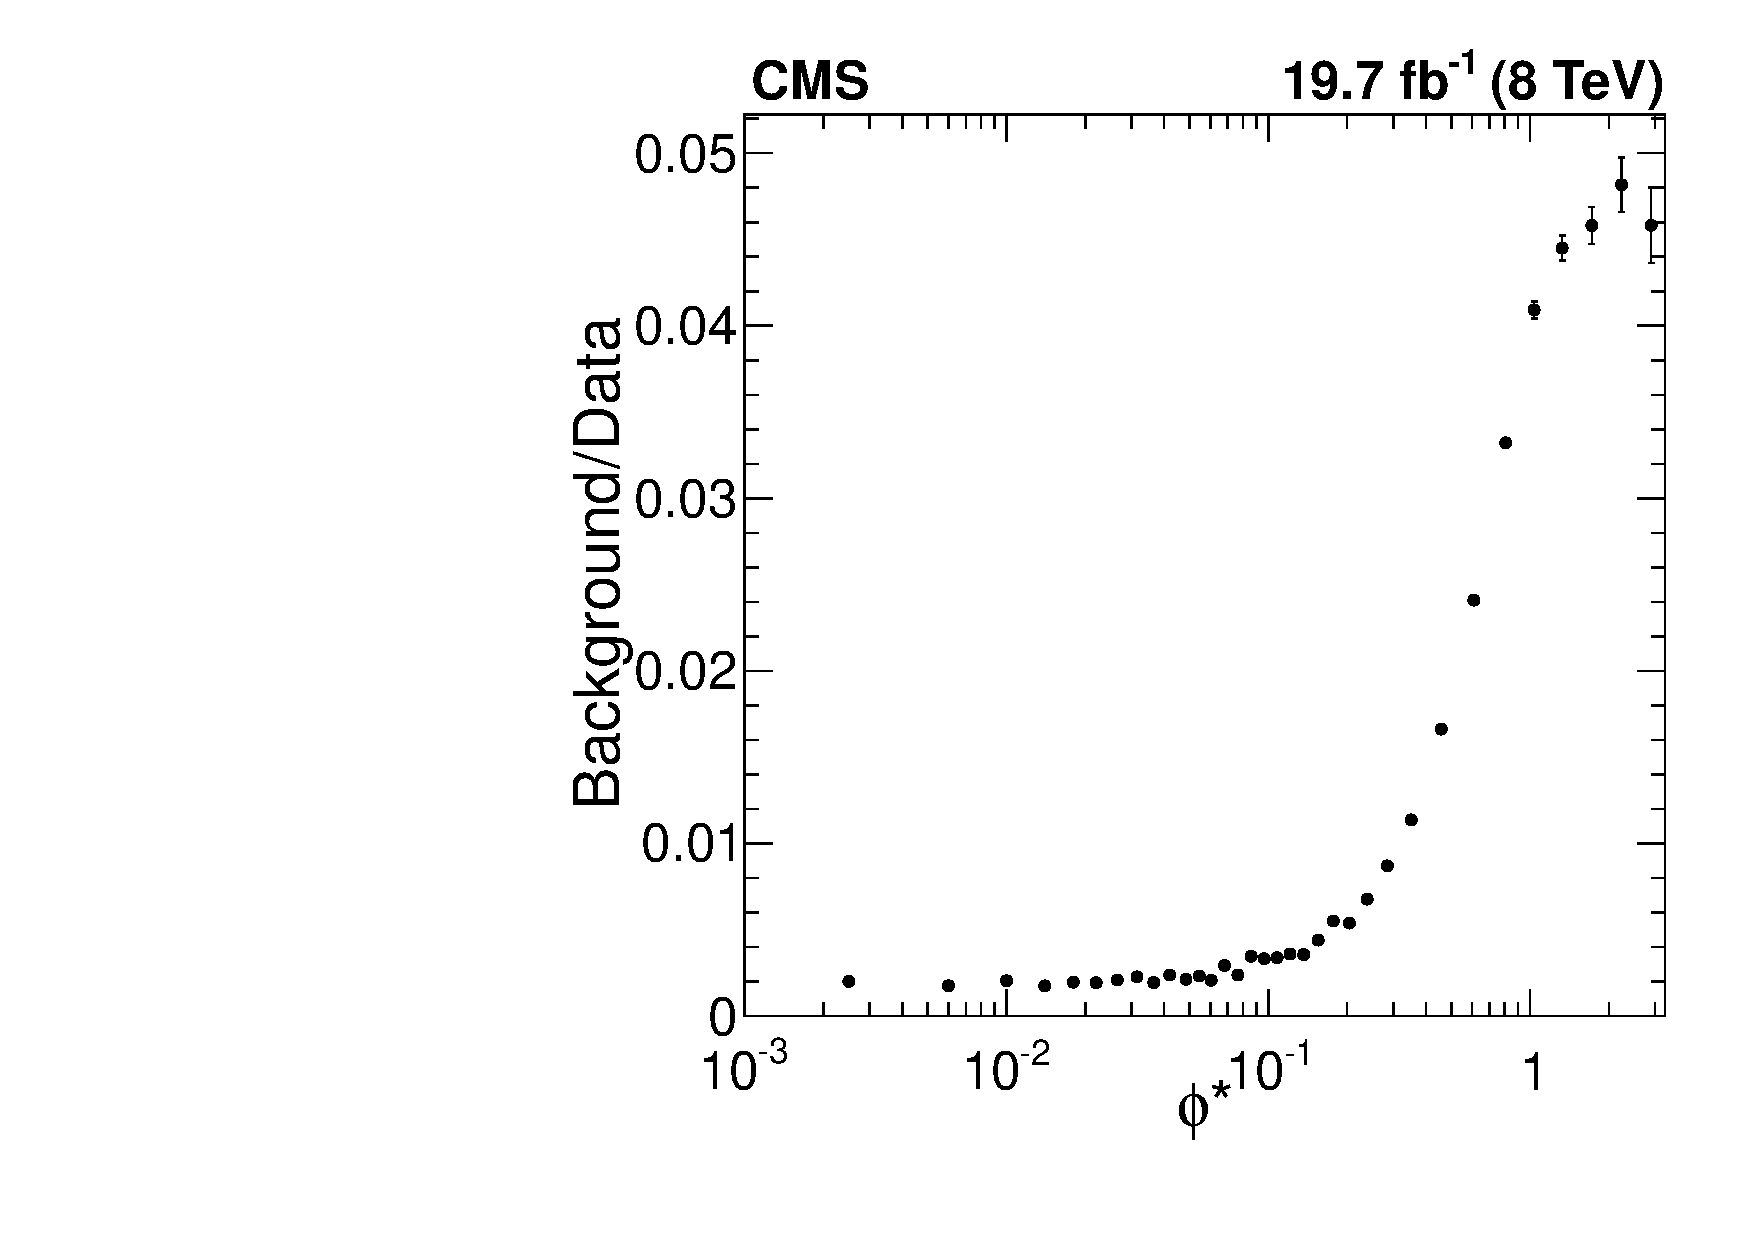
\includegraphics[width=\textwidth]{figures/DataSets/BGRatioMADGRAPHphistar.pdf}
    \caption[Background to data ratio]{Ratio of the background to data. This ratio grows by over a factory of 20 from  low to high \phistar  }
    \label{fig:PhistarDataVsBackground}
\end{figure}
\section{QCD Multi-jet and \texorpdfstring{$W^\pm+$}{W} jets}
QCD events are extremely common, happening at a rate of roughly 10 million times that of \Ztoee. Although QCD can not produce electrons directly, because electrons lack color charge, it does produce hadrons that can then produce electrons when the hadrons decay such as $\text{b}\rightarrow \text{c}+\text{W}^{-} \rightarrow \text{c+e}^{-}+\bar{\nu}$. Therefore QCD can produce them at a large rate. However, the selections made on electrons, described in the previous chapter, remove the vast majority of these QCD events leaving roughly only 1 in  10 billion making it into the final data sample. To successfully estimate the background rate due to these QCD events an impractically-large simulation sample for this analysis would be required. Thus a data-driven method is used to approximate the rate of QCD events for each \phistar bin individually.  

The data-driven method that is used takes advantage of the fact that QCD events generate electrons independently of each other. Therefore it is possible to do a study on events that produce either $e^-e^-$ or $e^+e^+$, which are referred to as same sign events. These events happen at the same rate as \xxpm{e}{e}. Consequently, by calculating the rate of  same sign events, the rate of opposite sign events is known. 

A collection of events was created from data using reconstructed electrons with the same sign, and passing all the same requirements used in the main analysis, except for \mee, as outlined in Chapter \ref{Chap:Efficiency}. The same requirements were placed on each simulation, as well as weighting them to the proper luminosity. The simulations used were the same as those that were used for the analysis itself. By requiring same sign events, most background and signal events in the simulation could be discarded, though some of the backgrounds were capable of creating a same sign pair that pass the requirements. These include ZZ, $W^{\pm}Z$, and even $\xxbar{t}{t}$ which could produce an electron from a jet. Other events, such as signal events could be kept if one of the two charges of the electron pair was misidentified. In fact because the Z cross-section is so large compared to the others, even though the vast majority of Z events were removed, there is still a noticeable amount of Z events in the final selection.  These weighted events are then separated into their respective \phistar bin and a \mee plot is created. The following function is then fit to the data:



\begin{equation}\label{eq:qcd_fit_function}
    \alpha \, \MCTemplate + \beta \, \BGFuncArgs.
\end{equation}
Where $T_{MC}$ comes directly from the simulations and $F_{BG}$ is a function that represents the QCD rate. The QCD function used in this analysis is:
\begin{equation}\label{eq:haupt_function}
    \BGFuncArgs = e^{- \gamma x} \erfc \left( \frac{\varepsilon - x}{\delta} \right).
\end{equation}
The free fit parameters are $\alpha$, $\beta$, $\gamma$, $\varepsilon$, and $\delta$. The resulting function is then integrated over the mass range of the analysis($\SI{60}{GeV}<m_{\text{ee}}<\SI{120}{GeV}$) and multiplied by two to compensate for the lack of charge requirements in the main analysis. However, due to a limited number of events in the bins and a high uncertainty for the fit, there are large jumps in the QCD values for each \phistar bin that are not physical. Therefore, the total distribution is smoothed by averaging each bin with its neighbors. The final uncertainty of this distribution is  set to 100\%. Two examples fits are shown in Fig. \ref{fig:QCDExampleCalc}.
\begin{figure}[!p]
    \centering
    \begin{subfigure}[b]{0.49\textwidth}
     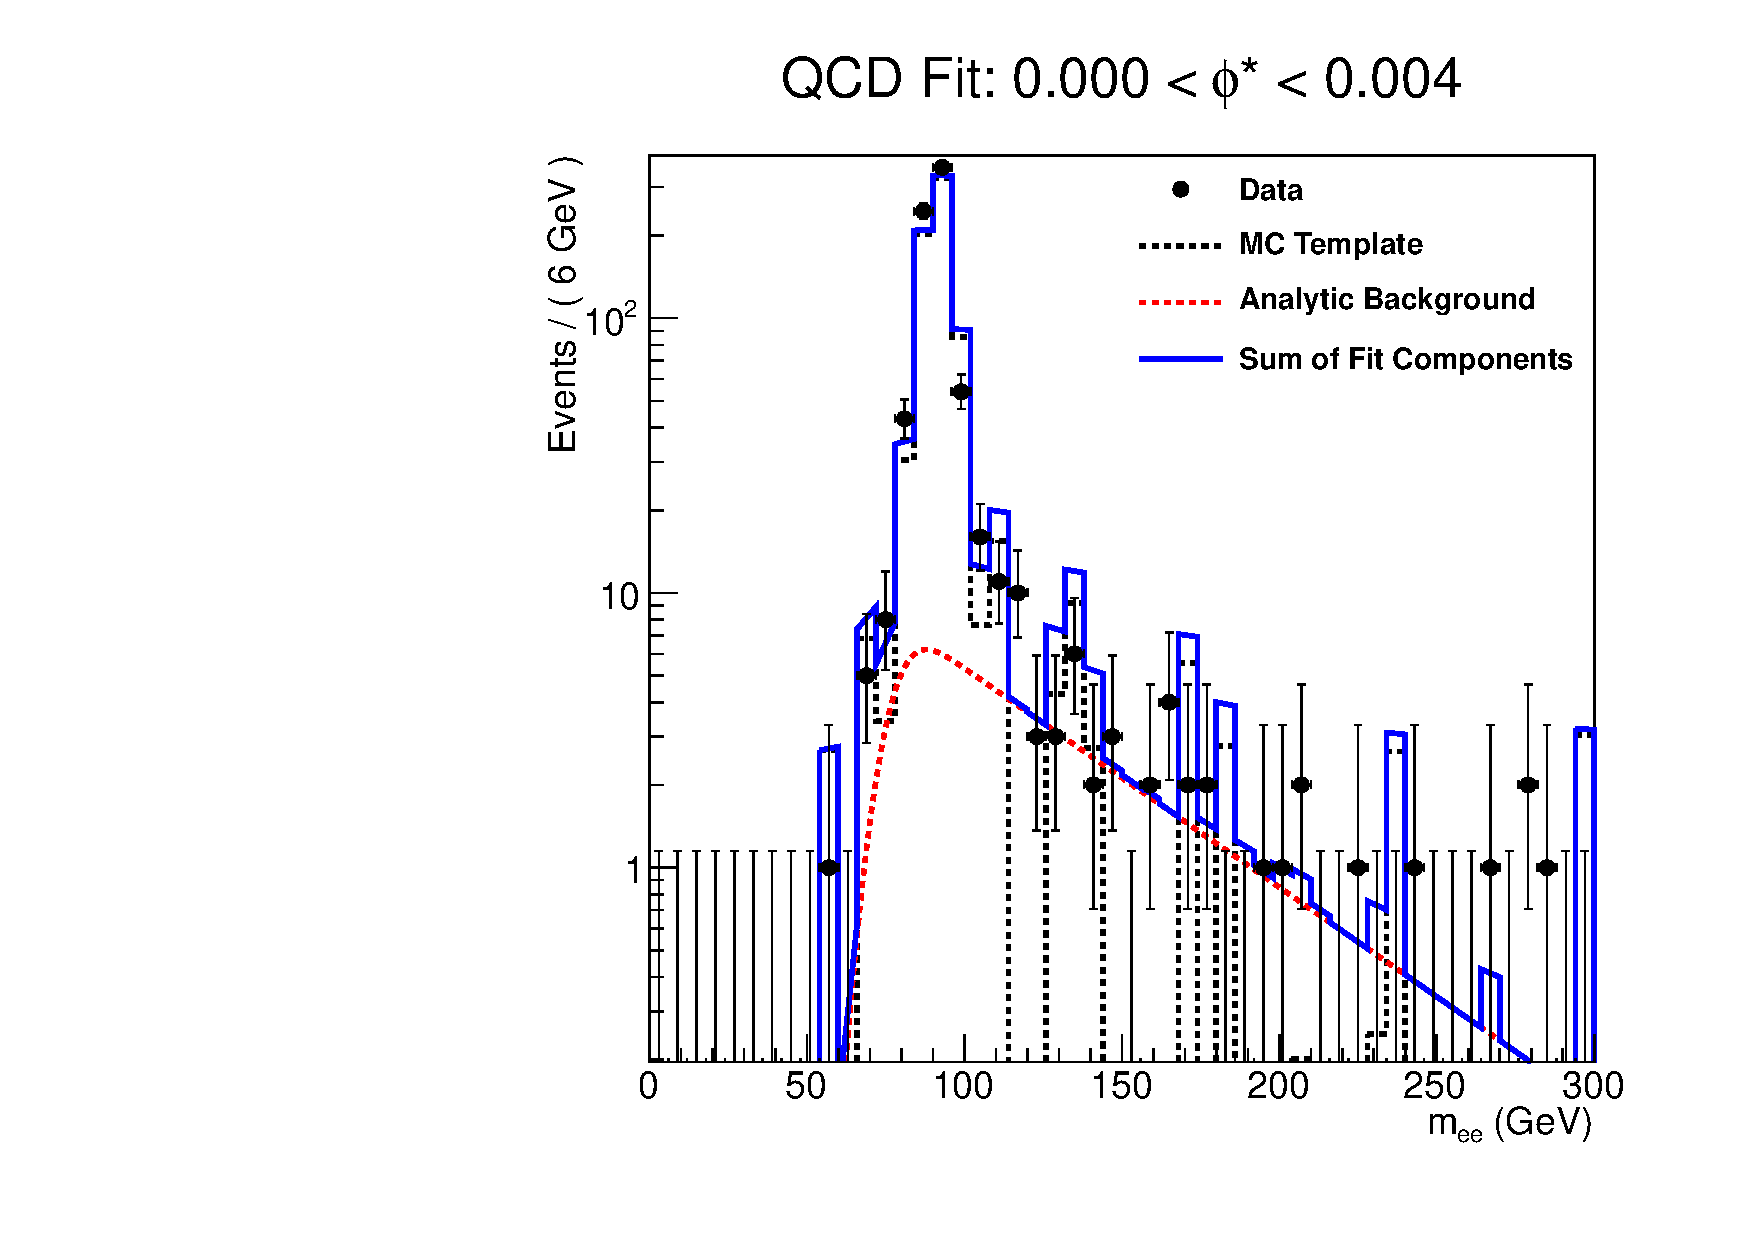
\includegraphics[width=\linewidth]{figures/DataSets/qcd_fit_plot_for_01.pdf}
     \caption{}
    \end{subfigure}
    \begin{subfigure}[b]{0.49\textwidth}
     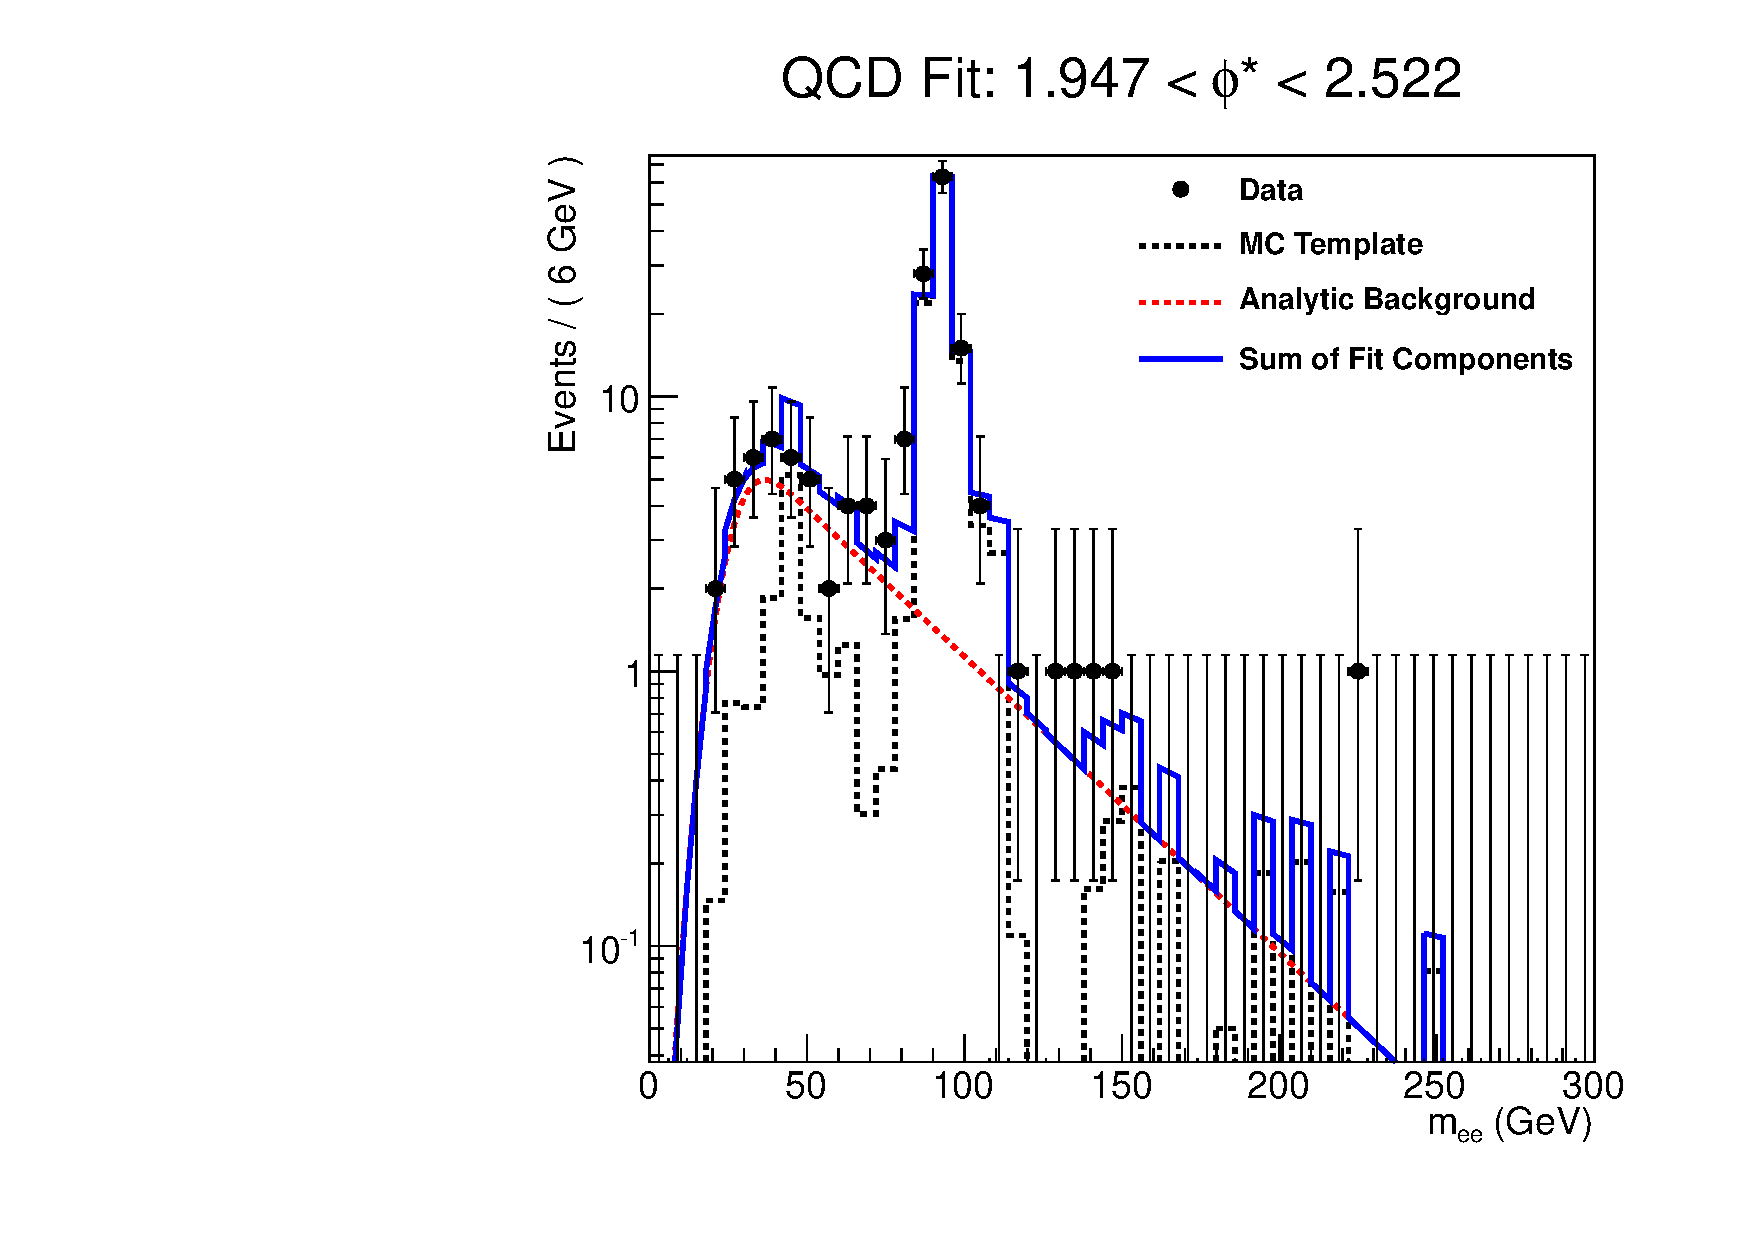
\includegraphics[width=\linewidth]{figures/DataSets/qcd_fit_plot_for_33.pdf}
     \caption{}
    \end{subfigure}
    \caption[QCD Fit examples]{QCD Fit examples from the first and final \phistar bins. As can be seen from the plot there still exist a Z peak due to misidentification of charge for some \Ztoee events. The QCD is taken as the integral of the fitting function from 60 to 120 GeV.}
    \label{fig:QCDExampleCalc}
\end{figure}
%%%%%%%%%%%%%%%%%%%%%%%%%%%%%%%%%%%%%%%%%%%%%%%%%%%%%%%%%%%%%%%%%%%%%%%%%%%%%%%%

%%%%%%%%%%%%%%%%%%%%%%%%%%%%%%%%%%%%%%%%%%%%%%%%%%%%%%%%%%%%%%%%%%%%%%%%%%%%%%%%
